\documentclass{article}
\usepackage{geometry}
\usepackage{graphicx}
\usepackage{amsmath}
\usepackage{algorithm}
\usepackage{algpseudocode}
\usepackage{multicol}
\usepackage{multirow}
\usepackage{arydshln}
\usepackage[usenames, dvipsnames]{color}
\geometry{
a4paper,
right=10mm,
left=10mm,
top=5mm,
bottom=5mm,	
}
\newcommand\tab[1][5pt]{\hspace*{#1}} 
\newcommand\sep{\tab | \tab } 
\begin{document}

\pagenumbering{gobble}

\begin{center}
\textbf{\huge Assignment 2 : CS335} \\
\textit{\Large Jayant Agrawal}         14282 \\
Section S1
\end{center}

\textbf{\huge Parsing}

\section*{Sol2: Parse Table}
The grammer: $G$ has the following productions(numbered):
\begin{enumerate}
\item $S \rightarrow Ma$
\item $S \rightarrow bMc$
\item $S \rightarrow dc$
\item $S \rightarrow bda$
\item $M \rightarrow d$
\end{enumerate}
Adding the production $S' \rightarrow S$ to get augmented grammer $G'$ and computing \emph{Sets-of-items}(Figure \ref{soi}):
\begin{figure}[h!]
\begin{multicols}{2}
\begin{equation*}
\begin{aligned}
I_0 &: S' \rightarrow .S  \\
&: S \rightarrow .Ma \hspace{5pt} | \tab .bMc \tab | \tab .dc \tab | \tab .bda \\
&: M \rightarrow .d
\end{aligned}
\end{equation*}

\begin{equation*}
\begin{aligned}
I_1 : goto(I_0,S) &: S' \rightarrow S.  \\
\end{aligned}
\end{equation*}


\begin{equation*}
\begin{aligned}
I_2 : goto(I_0,M) &: S \rightarrow M.a  \\
\end{aligned}
\end{equation*}


\begin{equation*}
\begin{aligned}
I_3 : goto(I_2,a) &: S \rightarrow Ma.  \\
\end{aligned}
\end{equation*}


\begin{equation*}
\begin{aligned}
I_4 : goto(I_0,b) &: S \rightarrow b.Mc \tab | \tab b.da  \\
&: M \rightarrow .d \\
\end{aligned}
\end{equation*}


\begin{equation*}
\begin{aligned}
I_5 : goto(I_4,M) &: S \rightarrow bM.c  \\
\end{aligned}
\end{equation*}


\begin{equation*}
\begin{aligned}
I_6 : goto(I_4,d) &: S \rightarrow bd.a  \\
&: M \rightarrow d.  \\
\end{aligned}
\end{equation*}

\begin{equation*}
\begin{aligned}
I_7 : goto(I_5,c) &: S \rightarrow bMc.  \\
\end{aligned}
\end{equation*}

\begin{equation*}
\begin{aligned}
I_8 : goto(I_6,a) &: S \rightarrow bda.  \\
\end{aligned}
\end{equation*}

\begin{equation*}
\begin{aligned}
I_9 : goto(I_0,d) &: S \rightarrow d.c  \\
&: M \rightarrow d.  \\
\end{aligned}
\end{equation*}


\begin{equation*}
\begin{aligned}
I_{10} : goto(I_9,c) &: S \rightarrow dc.  \\
\end{aligned}
\end{equation*}
\end{multicols}
\caption{Sol2: Sets-of-items}
\label{soi}
\end{figure}

Also, the first and follow sets of the non-terminals in $G$ are as follows:\\
first(S) = \{b,d\}\\
first(M) = \{d\} \\
follow(S) = \{\$\} \\
follow(M) = \{a,c\} \\ \\
Using the above first, follow sets and the sets-of-items, we get the following SLR Parse Table (Figure \ref{slr} ) :
\begin{figure}[h!]
\begin{center}
\begin{tabular}{||c | c c c c c | c c||}
\hline
\hline
\multirow{2}{*}{\textbf{STATE}} & \multicolumn{5}{c|}{\emph{action}}  & \multicolumn{2}{c||}{\emph{goto}} \\
\cline{2-8}
& \bf a & \bf b & \bf c & \bf d & \$ & \bf S &\bf M \\
\hline
0 & & {\color{ForestGreen} s4} & & {\color{ForestGreen} s9} & & 1 &2 \\
\hdashline[0.5pt/10pt]
1 & & & & & {\color{red} \emph{acc}} &  & \\
\hdashline[0.5pt/10pt]
2 &{\color{ForestGreen} s3} &  & &  & &  & \\
\hdashline[0.5pt/10pt]
3 & & & & & {\color{blue} r1} &  & \\
\hdashline[0.5pt/10pt]
4 & & & & {\color{ForestGreen} s6} &  &  & 5\\
\hdashline[0.5pt/10pt]
5 & & & {\color{ForestGreen} s7}& &  &  & \\
\hdashline[0.5pt/10pt]
6 & \begin{tabular}{c} {\color{ForestGreen} s8} \\ {\color{blue} r5} \end{tabular} & & {\color{blue} r5}& &  &  & \\
\hdashline[0.5pt/10pt]
7 &  & & & & {\color{blue} r5} &  & \\
\hdashline[0.5pt/10pt]
8 &  & & & & {\color{blue} r4} &  & \\
\hdashline[0.5pt/10pt]
9 & {\color{blue} r5} & &\begin{tabular}{c} {\color{ForestGreen} s10} \\ {\color{blue} r5} \end{tabular} & &  &  & \\
\hdashline[0.5pt/10pt]
10 &  & & & & {\color{blue} r5} &  & \\
\hline
\hline
\end{tabular}
\end{center}
\caption{Sol2: SLR Parse Table}
\label{slr}
\end{figure}
\newpage
\section*{Sol3: SLR vs CLR vs LALR}
Consider the Sets-of-items (Figure \ref{soi3}) and Automation(Figure \ref{auto3}) for the given grammer.
\begin{figure}[h!]
\begin{multicols}{2}
\begin{equation*}
\begin{aligned}
I_0 &: S' \rightarrow .S  \\
&: S \rightarrow .id[E] := E
\end{aligned}
\end{equation*}

\begin{equation*}
\begin{aligned}
I_1 : goto(I_0,id) &: S \rightarrow id.[E] :=E  \\
\end{aligned}
\end{equation*}

\begin{equation*}
\begin{aligned}
I_2 : goto(I_0,S) &: S' \rightarrow S.  \\
\end{aligned}
\end{equation*}

\begin{equation*}
\begin{aligned}
I_3 : goto(I_1,[) &: S \rightarrow id[.E] :=E  \\
&: E \rightarrow .E+T \tab | \tab .T \\
&: T \rightarrow .T*F \tab | \tab  .F \\
&: F \rightarrow .(E) \sep .id \\
\end{aligned}
\end{equation*}

\begin{equation*}
\begin{aligned}
I_4 : goto(I_3,() &: F \rightarrow (.E)  \\
&: E \rightarrow .E+T \tab | \tab .T \\
&: T \rightarrow .T*F \tab | \tab  .F \\
&: F \rightarrow .(E) \sep .id \\
\end{aligned}
\end{equation*}

\begin{equation*}
\begin{aligned}
I_5 : goto(I_3,id) &: F \rightarrow id.  \\
\end{aligned}
\end{equation*}

\begin{equation*}
\begin{aligned}
I_6 : goto(I_3,E) &: S \rightarrow id[E.] :=E  \\
&: E \rightarrow E.+T \\
\end{aligned}
\end{equation*}

\begin{equation*}
\begin{aligned}
I_7 : goto(I_6,]) &: S \rightarrow id[E]. :=E  \\
\end{aligned}
\end{equation*}

\begin{equation*}
\begin{aligned}
I_8 : goto(I_6,+) &: E \rightarrow E+.T  \\
&: T \rightarrow .T*F \tab | \tab  .F \\
&: F \rightarrow .(E) \sep .id \\
\end{aligned}
\end{equation*}


\begin{equation*}
\begin{aligned}
I_9 : goto(I_3,T) &: E \rightarrow T.  \\
&: T \rightarrow T.*F  \\
\end{aligned}
\end{equation*}

\begin{equation*}
\begin{aligned}
I_{10} : goto(I_9,*) &: T \rightarrow T*.F  \\
&: F \rightarrow .(E) \sep .id
\end{aligned}
\end{equation*}


\begin{equation*}
\begin{aligned}
I_{11} : goto(I_3,F) &: T \rightarrow F.  \\
\end{aligned}
\end{equation*}


\begin{equation*}
\begin{aligned}
I_{12} : goto(I_4,E) &: F \rightarrow (E.)  \\
&: E \rightarrow E.+T 
\end{aligned}
\end{equation*}


\begin{equation*}
\begin{aligned}
I_{13} : goto(I_{12},)) &: F \rightarrow (E).  \\
\end{aligned}
\end{equation*}


\begin{equation*}
\begin{aligned}
I_{14} : goto(I_8,T) &: E \rightarrow E+T.  \\
&: T \rightarrow T.*F
\end{aligned}
\end{equation*}

\begin{equation*}
\begin{aligned}
I_{15} : goto(I_7,:=) &: S \rightarrow id[E] := .E  \\
&: E \rightarrow .E+T \tab | \tab .T \\
&: T \rightarrow .T*F \tab | \tab  .F \\
&: F \rightarrow .(E) \sep .id \\
\end{aligned}
\end{equation*}

\begin{equation*}
\begin{aligned}
I_{16} : goto(I_{10},F) &: T \rightarrow T*F.
\end{aligned}
\end{equation*}


\begin{equation*}
\begin{aligned}
I_{17} : goto(I_{15},E) &: S \rightarrow id[E] := E. \\
&: E \rightarrow E.+T \\
\end{aligned}
\end{equation*}

\begin{equation*}
\begin{aligned}
I_{9} &: goto(I_4,T) \\
I_8 &: goto(I_{12},+) \\
\color{red} {I_4} &: \color{red} {goto(I_{4},( \tab )} \\
I_5 &: goto(I_{4},id) \\
I_{11} &: goto(I_{4},F) \\
I_{10} &: goto(I_{14},*) \\
I_{11} &: goto(I_{8},F) \\ 
I_{4} &: goto(I_{8},C) \\
I_{10} &: goto(I_{9},*) \\
I_{5} &: goto(I_{8},id) \\
I_{4} &: goto(I_{10},( \tab ) \\
I_{5} &: goto(I_{15},id) \\
I_{9} &: goto(I_{15},T) \\
I_{11} &: goto(I_{15},F) \\
I_{4} &: goto(I_{15},( \tab ) \\
I_{8} &: goto(I_{17},+) \\
I_{5} &: goto(I_{10},id) \\
\end{aligned}
\end{equation*}
\end{multicols}
\caption{Sol3: LR(0) Sets-of-items }
\label{soi3}
\end{figure}

\begin{figure}[h!]
\begin{center}
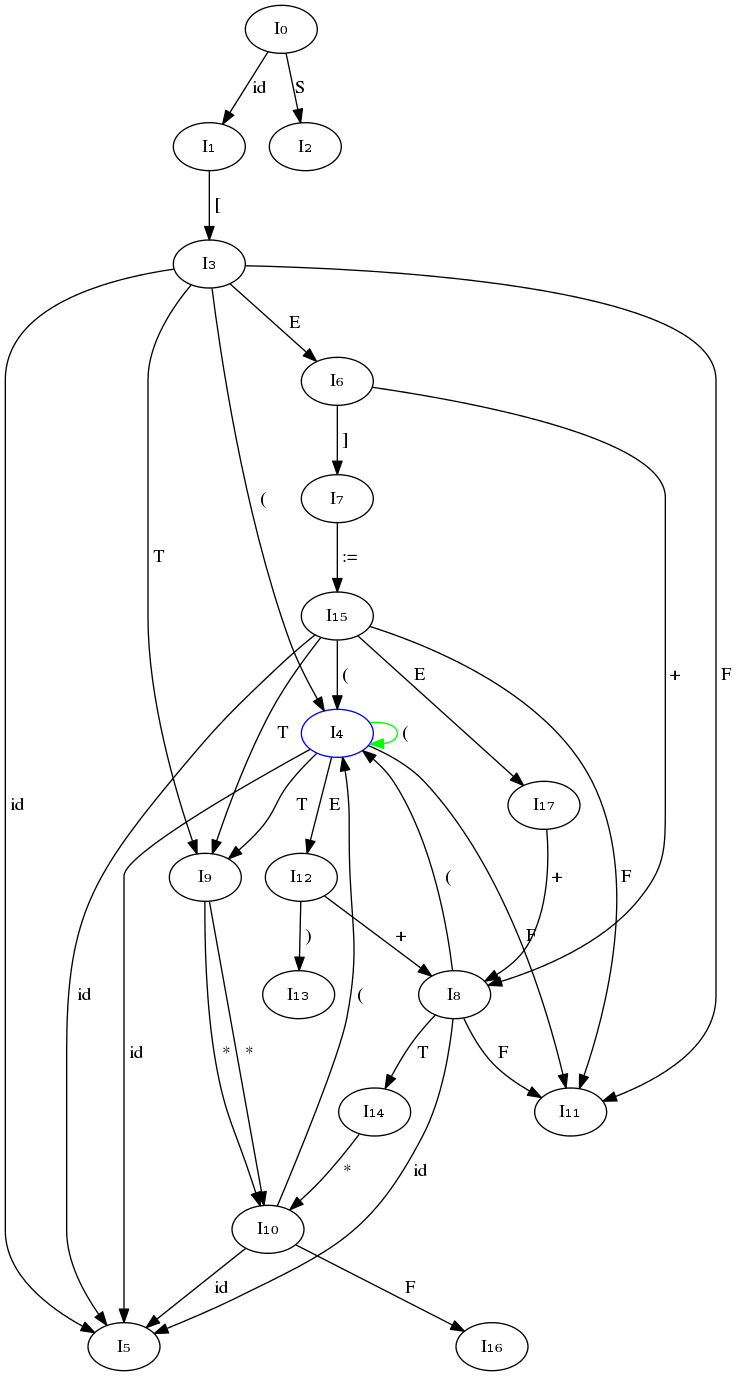
\includegraphics[scale=0.5]{autoSLR.png}
\caption{Sol3: Automation SLR }
\label{auto3}
\end{center}
\end{figure}

\end{document}



